\documentclass{beamer}
%\usepackage[utf8]{inputenc}
\usepackage[greek,english]{babel}
\usepackage{fontspec}
\usepackage{xunicode}
\usepackage{xltxtra}
\setromanfont{FreeSerif}
\setsansfont{FreeSans}
\setmonofont{FreeMono}
\setmainfont{DejaVuSans}
\usetheme{Warsaw}
\title[The Wikipedia Case]{The Wikipedia Case\\How does Wikipedia work?}
\author{Alexandros Kosiaris}
\date{May 20, 2014}
\begin{document}

\begin{frame}
\titlepage
\end{frame}

\AtBeginSubsection[]
{
 \begin{frame}<beamer>
   \frametitle{Layout}
   \tableofcontents[currentsection,currentsubsection]
 \end{frame}
}

\section{Outline}
\frame{\tableofcontents}

\section{Introduction}
\begin{frame}{Disclaimer}
	\begin{beamercolorbox}[center,shadow=true,rounded=true,]{note}
	Any views or opinions presented are solely those of the author/presenter and do not necessarily
	represent those of Wikimedia Foundation, any Wikipedia user group, community or any other entity
	aside from his own
	\end{beamercolorbox}
\end{frame}
\begin{frame}{What is Wikipedia}
	\begin{itemize}
		\pause \item Wikipedia is a collaboratively edited, multilingual, free Internet encyclopedia
		\pause \item Supported by the non-profit Wikimedia Foundation
		\pause \item Volunteers worldwide collaboratively write Wikipedia's 30 million articles in 287 languages
		\pause \item Including over 4.5 million in the English Wikipedia
		\pause \item \emph{Anyone who can access the site can edit almost any of its articles}
	\end{itemize}
\end{frame}
\begin{frame}{Wiki}
	Wiki ? What is a Wiki?
	\begin{itemize}
		\pause \item Hawaian for "quick"
		\pause \item A wiki is a web application which allows people to add, modify, or delete content in collaboration
			with others. In a typical wiki, text is written using a simplified markup language or a rich-text editor
	\end{itemize}
	\pause So a portmanteau of \emph{wiki} and \emph{encyclopedia}
\end{frame}
\begin{frame}{Does it work?}
	\begin{itemize}
		\pause \item In February 2014, The New York Times reported that Wikipedia is ranked 5th globally among all websites
		\pause \item 18 billion page views and nearly 500 million unique visitors per month
		\pause \item Wikipedia trails just Yahoo, Facebook, Microsoft and Google, the largest having 1.2 billion unique visitors
	\end{itemize}
	\pause
	So it \emph{DOES} work
\end{frame}

\section{Wikipedia Origins}
\begin{frame} {Early Start}
	Predecessor:
	\begin{itemize}
		\pause \item 2000: In March Jimmy Wales founded Nupedia, a free online encyclopaedia
		\pause \item Larry Sanger as editor in chief.
		\pause \item Nupedia was organized like existing encyclopaedias, with an advisory board of experts and a lengthy review process.
		\pause \item By January 2001 fewer than two dozen articles were finished
		\pause \item Sanger advocated supplementing Nupedia with an open-source encyclopaedia based on wiki software.
	\end{itemize}
\end{frame}

\begin{frame} {Early Starts (2)}
	First Steps:
	\begin{itemize}
		\pause \item On Jan. 15, 2001, Wikipedia was launched as a feature of Nupedia.com
		\pause \item Relaunched as independent Web site a few days later
		\pause \item In its first year Wikipedia expanded to some 20,000 articles in 18 languages
		\pause \item In 2003 Nupedia was terminated and its articles moved into Wikipedia
		\pause \item English Wikipedia passed the mark of two million articles on September 9, 2007, making it the
			largest encyclopedia ever assembled
	\end{itemize}
\end{frame}

\begin{frame} {Success stories}
	Growth:
	\begin{itemize}
		\pause \item Around 1,800 articles were added daily to the encyclopedia in 2006
		\pause \item In January 2007, Wikipedia entered for the first time the top-ten list of the most popular websites in the United States
		\pause \item With 42.9 million unique visitors, Wikipedia was ranked number 9
		\pause \item In February 2014, a global monthly total of over 12 billion pageviews
		\pause \item 5th most popular website
		\pause \item Participated in protests against Stop Online Piracy Act and PROTECT IP Act. 162 million people witnessed the blackout explanation page
	\end{itemize}
\end{frame}

\section{Operation}
\begin{frame} {WMF}
	Wikipedia is hosted and funded by the Wikimedia Foundation
	\begin{itemize}
		\pause \item A non-profit organization
		\pause \item Relies on public contributions and grants to fund its mission
		\pause \item Responsible for a number of other projects as well
		\pause \item wikinews, wikiversity, wikidata, wikivoyage, wikibooks, wikispecies, etc
		\pause \item Various chapters exist (WMDE, WMCH, etc)
	\end{itemize}
\end{frame}

\begin{frame} {Funding}
	How does WMF survive?
	\begin{itemize}
		\pause \item Strictly through public contributions and grants
		\pause \item Very important about remaining unbiased and having a neutral point of view
		\pause \item Revenue: 39.7 million
		\pause \item Expenses: 29 million
		\pause \item Assets: 37.2 million
		\pause \item Liabilities: 2.3 million.
	\end{itemize}
\end{frame}

\begin{frame} {Funding 2}
	An example of banner for public contribution:
	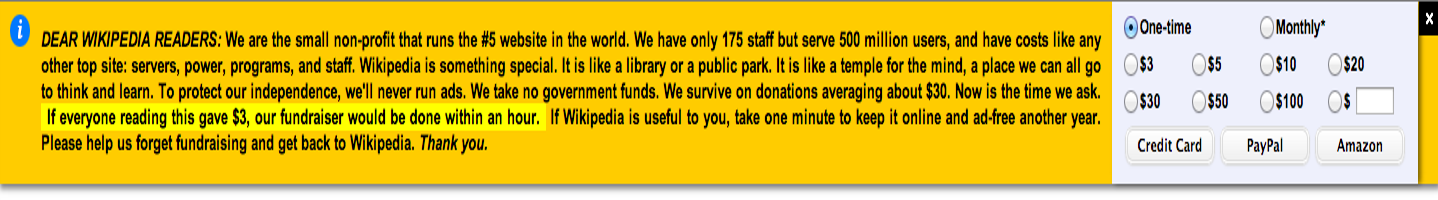
\includegraphics[width=\linewidth]{Goldbanner.png}
	\begin{itemize}
		\pause \item Note the amounts
	\end{itemize}

\end{frame}

\begin{frame} {Software}
	Note the pattern:
	\begin{itemize}
		\pause \item Mediawiki: Free and/or Open Source wiki software written in PHP and built upon MySQL
		\pause \item Varnish: Free and/or Open Source reverse caching proxy
		\pause \item Apache: Free and/or Open Source Web Server
		\pause \item PHP: Free and/or Open Source language
		\pause \item MySQL: Free and/or Open Source relational database system
		\pause \item ElasticSearch: Free and/or Open Source NoSQL, search friendly database
		\pause \item LVS: Free and/or Open Source load balancing framework
		\pause \item Ubuntu Linux: Free and/or Open Source Operating System
	\end{itemize}
\end{frame}

\begin{frame}{Free and/or Open Source Software}
	What is Free and/or Open Source Software?
	\begin{itemize}
		\pause \item Anyone is freely licensed to:
			\begin{itemize}
				\pause \item use
				\pause \item copy
				\pause \item study
				\pause \item change the software in any way
			\end{itemize}
		\pause \item The source code is openly shared so that people are encouraged to voluntarily improve the design of the software
	\end{itemize}
\end{frame}

\begin{frame} {Content Access}
	Ways of accessing the content:
	\begin{itemize}
		\pause \item Website
		\pause \item Mobile Apps (Apple Store, Google Play, etc)
		\pause \item Search Engines (Google Knowledge Graph, Bing)
		\pause \item Compact Discs, DVDs, USB sticks
		\pause \item Books
		\pause \item Publicly available dumps of almost everything
	\end{itemize}
\end{frame}

\begin{frame} {Edit Access}
	Ways of editing the content:
	\begin{itemize}
		\pause \item Website
		\pause \item Mobile Apps (Apple Store, Google Play, etc)
	\end{itemize}
\end{frame}

\section{Nature}
\begin{frame} {Editing}
	Editing:
	\begin{itemize}
		\pause \item Unlike traditional encyclopedias, Wikipedia allows outside editing
		\pause \item \emph{I CAN EDIT}
		\pause \item \emph{YOU CAN EDIT}
		\pause \item \emph{ANYONE CAN EDIT}
		\pause \item Even anonymously
		\pause \item Except in particularly sensitive and/or vandalism-prone pages that are "protected"
		\pause \item But the policy can be changed depending on language. So no new anonymous articles on en.wikipedia.org
	\end{itemize}
\end{frame}
\begin{frame} {Editing (2)}
	Editing:
	\begin{itemize}
		\pause \item No article is considered to be owned by its creator or any other editor
		\pause \item Nor is it vetted by any recognized authority.
		\pause \item Editors are supposed to agree on the content and structure of articles by consensus.
		\pause \item Any change can be reverted
		\pause \item So discuss stuff (through the Talk page)
	\end{itemize}
\end{frame}

\begin{frame} {Talk page}
	A Talk page example
	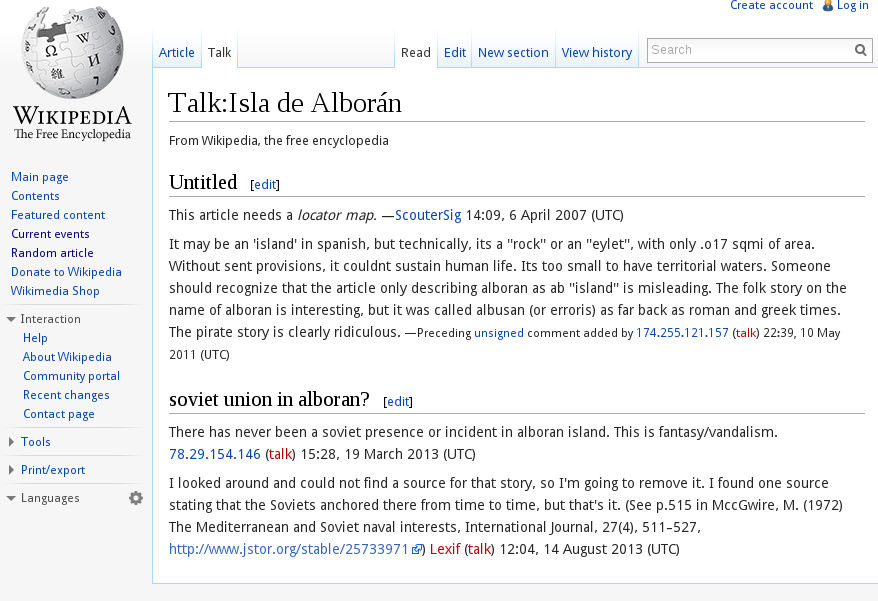
\includegraphics[height=7.8cm]{Talkpage.png}
\end{frame}

\subsection{Policy}
\begin{frame}{Rules and guidelines}
	The are rules and guidelines
	\begin{itemize}
		\pause \item Neutral point of view
			\begin{itemize}
				\pause \item Remain unbiased
				\pause \item Do not use language that favor a point of view
			\end{itemize}
		\pause \item No original research
		\pause \item Reliable published sources must exist
		\pause \item Verifiability
			\begin{itemize}
				\pause \item Citation needed
			\end{itemize}
	\end{itemize}
\end{frame}
\begin{frame}{Rules and guidelines (2)}
	The are rules and guidelines (2)
	\begin{itemize}
		\pause \item Biographies of living persons
			\begin{itemize}
				\pause \item Possible but extra care must be taken to not victimize and/or violate privacy
			\end{itemize}
		\pause \item Libel
			\begin{itemize}
				\pause \item A sure way to get blocked and have edit revert
			\end{itemize}
		\pause \item Wikipedia is not a dictionary
			\begin{itemize}
				\pause \item Not just a definition but also other content
				\pause \item Go to wictionary!
			\end{itemize}
		\pause \item No autobiographies please. No way you can be partial and unbiased
	\end{itemize}
\end{frame}
\begin{frame}{Conflict of interest}
	What is conflict of interest?
	\pause When an external relationship undermines, or could reasonably be said to undermine, your role as a Wikipedian, you have a conflict of interest.
	\pause So no:
	\begin{itemize}
		\pause \item Getting paid for an article
		\pause \item Getting paid to promote someone/something on wikipedia
		\pause \item Self-promotion
		\pause \item Writing about one's own circle (family, friends, colleagues)
		\pause \item Citing oneself
	\end{itemize}
\end{frame}

\begin{frame}{More guidelines}
	And more of this:
	\begin{itemize}
		\item Child protection
		\item Civility
		\item Consensus
		\item Edit warring (including the three-revert rule)
		\item Harassment
		\item No legal threats
		\item No personal attacks
		\item No ownership of articles
		\item Sock puppetry
		\item Vandalism
	\end{itemize}

	The full list at:
	\beamerbutton{https://en.wikipedia.org/wiki/Wikipedia:List\_of\_policies\_and\_guidelines}
\end{frame}

\begin{frame}{Copyright and License}
	Copyright:
		\begin{itemize}
			\pause \item Must respect copyright (so do not add stuff protected by copyright)
			\pause \item Editors/contributors have copyright
			\pause \item Content implicitly licensed under CC-BY-SA/GFDL
			\pause \item Essentially content is \emph{FREE} for everyone
		\end{itemize}
\end{frame}

\begin{frame}{CC-BY-SA?}
	Creative Commons baselines rights for works of art
	\begin{itemize}
		\item Attribution     (BY)
		\item Share-alike	(SA)
		\item Non-commercial	(NC)
		\item Non-derivative	(ND)
	\end{itemize}
	\pause Resulting licenses
	\begin{itemize}
		\item Attribution alone	BY
		\item Attribution + NoDerivatives	BY-ND
		\item Attribution + ShareAlike		BY-SA
		\item Attribution + NonCommercial	BY-NC
		\item Attribution + NonCommercial + NoDerivatives	BY-NC-ND
		\item Attribution + NonCommercial + ShareAlike		BY-NC-SA
	\end{itemize}
\end{frame}
\begin{frame}{GFDL}
	GNU Free Documentation License
	\begin{itemize}
		\pause \item An older License that Wikipedia migrated from on 2009
		\pause \item Compatible with CC-BY-SA
		\pause \item Same principle, minor legal differences
	\end{itemize}
\end{frame}

\subsection{Community}
\begin{frame}{Size}
	Size:
	\begin{itemize}
		\pause \item Always referring to editors. Only volunteers!
		\pause \item In April 2008, estimation of 100M man-hours
		\pause \item In November 2011, there were approximately 31.7 million registered user accounts across all language editions
		\pause \item 270,000 accounts were active on a monthly basis.
		\pause \item October 2013, 31,000 editors are active on the English Wikipedia
		\pause \item About half of the active editors spend at least one hour a day editing, and a fifth spend more than three hours
	\end{itemize}
\end{frame}
\begin{frame}{Motivation}
	A survey in 2007 by Odev Nov studied the following driving concepts
	\begin{itemize}
		\pause \item Values – expressing values to do with altruism and helping others
		\pause \item Social – engaging with friends
		\pause \item Understanding – expanding knowledge through activities
		\pause \item Career – gaining work experience and skills
		\pause \item Protective – reducing guilt over personal privilege
		\pause \item Enhancement – demonstrating knowledge to others
		\pause \item Ideology – the belief that knowledge should be free
		\pause \item Fun – enjoying the activity
	\end{itemize}
	\pause The most common where: Fun, Ideology, Values. The least common: Career, Social, Protective
\end{frame}
\begin{frame}{Socializing}
	The communities socialize:
	\begin{itemize}
		\pause \item Wikimania conference
		\pause \item Wiknics
		\pause \item Wikimedia hackathon (Gather around and write/discuss code)
		\pause \item May or may not meet independently depending on the size/language/culture
		\pause \item Online: IRC or whatever else they feel like
	\end{itemize}
\end{frame}

\begin{frame}{Vandalism}
	It happens. Constantly. So how to fight it?
	\begin{itemize}
		\pause \item It is programmatically easy to spot some kinds of vandalism (spam, advertising)
		\pause \item Bots to the rescue!
		\pause \item Selected volunteers with extra privileges
			\begin{itemize}
				\pause \item Administrators (per wiki/language)
				\pause \item Bureaucrats (per wiki/language)
				\pause \item Stewards (global)
				\pause \item Reviewers, rollbacks, file movers, confirmed users,oversights
			\end{itemize}
	\end{itemize}
\end{frame}
\begin{frame} {Bots}
	Bot ? What is a bot ?
	\begin{itemize}
		\pause \item Short for robot
		\pause \item Software programs performing copius and repetetive tasks such:
			\begin{itemize}
				\pause \item Fixing syntax errors
				\pause \item Removing spam
				\pause \item Fixing style
				\pause \item Even automatically start articles
			\end{itemize}
		\pause \item Bots \emph{MUST} be pre-approved!
	\end{itemize}
\end{frame}

\begin{frame}{Administrators}
	The English Wikipedia currently has currently 1,409 administrators. These are selected editors that:
	\begin{itemize}
		\pause \item Ask for it and are approved after a consensus
		\pause \item Have the rights to use extra tools like:
			\begin{itemize}
				\pause \item Page deletion
				\pause \item Page protection
				\pause \item User/IP blocking and unblocking
				\pause \item Tools to modify fully protected pages and the Mediawiki interface
				\pause \item Grant and revoke rights to other users
			\end{itemize}
	\end{itemize}
\end{frame}
\begin{frame}{Bureaucrats}
	The English Wikipedia currently has currently 35 bureaucrats
	Exceptionally trusted and selected editors that:
	\begin{itemize}
		\pause \item Ask for it and are approved after a consensus
		\pause \item Have the rights to:
			\begin{itemize}
				\pause \item Rename users
				\pause \item Grant and revoke Administrator/bot rights
				\pause \item Grant bureaucrat (but not remove)
			\end{itemize}
	\end{itemize}
\end{frame}
\begin{frame}{Stewards}
	There are 38 stewards in total.
	\begin{itemize}
		\pause \item Elected by the community
		\pause \item Have all the rights administrators/bureaucrats do plus:
			\begin{itemize}
				\pause \item Remove adminstrator/bureaucrat
			\end{itemize}
		\pause \item The idea is to have people that can in the absence of a strong local community perform necessary tasks.
		\pause \item Solve the chicken/egg problem
	\end{itemize}
\end{frame}

\begin{frame} {Dispute resolution}
	There will always be disputes
	\begin{itemize}
		\pause \item Editors try to resolve them amicably
		\pause \item Adding more arguments, citations, references, sources
		\pause \item Trying to avoid middle ground
			\begin{itemize}
				\pause \item There is no such thing as half-pregnant!
			\end{itemize}
		\pause \item Avoid Edit wars!
		\pause \item Bring third parties into the dispute: Other editors and/or Administrators
	\end{itemize}
\end{frame}

\begin{frame} {Arbitration Commitee}
	If nothing works, the Arbitration Commitee is to be contacted
	\begin{itemize}
		\pause \item Elected
		\pause \item Listen to arguments and takes a decision
		\pause \item Lasting a pre-specified amount of time
		\pause \item The English Wikipedia Arbritration Commitee has decided on 371 cases up to now:
		\pause \item Austrian Economics, Socionics, Longevity and Shakespeare, Church of Scientology
	\end{itemize}
\end{frame}

\section{Greek Wikipedia}
\begin{frame} {Some statistics}
	On May 2014 el.wikipedia.org had:
	\begin{itemize}
		\pause \item > 100000 articles
		\pause \item > 10000 uploaded files
		\pause \item > 145000 registered users
		\pause \item 824 active users
		\pause \item 95 bots, 22 Administrators, 3 bureaucrats
	\end{itemize}
\end{frame}
\begin{frame} {Some Graphs}
	Let's skip to a browser!
\end{frame}
\begin{frame} {Popular pages}
	On March 2014 some of the most popular pages were:
	\begin{itemize}
		\pause \item System pages (main page, random page, etc) ( > 1M page views)
		\pause \item Αυτόνομη Δημοκρατία της Κριμαίας (85668 page views)
		\pause \item Χρήστης:Diu (70392 page views)
		\pause \item User:Diu (64897 page views)
		\pause \item Ελληνική Επανάσταση του 1821 (63690 page views)
		\pause \item Ισημερία (55995 page views)
		\pause \item Ουκρανία (46495 page views)
	\end{itemize}
\end{frame}
\begin{frame} {The Greek Community}
	\begin{itemize}
		\pause \item Not well organized, used to be not very large/active
		\pause \item 2013 Wikimedia Community User Group Greece officialy recognized (1 year, to be extended)
		\pause \item 100000 articles now!
		\pause \item Κατσανέβας vs User:Diu Court case
	\end{itemize}
\end{frame}

\section{Questions}
\begin{frame}{Disclaimer}
	\begin{beamercolorbox}[center,shadow=true,rounded=true,]{note}
	Any views or opinions presented are solely those of the author/presenter and do not necessarily
	represent those of Wikimedia Foundation, any Wikipedia user group, community or any other entity
	aside from his own
	\end{beamercolorbox}
\end{frame}

\begin{frame}{Questions}
	\begin{beamercolorbox}[center,shadow=true,rounded=true,]{note}
		        Questions?
	\end{beamercolorbox}
\end{frame}

\end{document}
